
%(BEGIN_QUESTION)
% Copyright 2011, Tony R. Kuphaldt, released under the Creative Commons Attribution License (v 1.0)
% This means you may do almost anything with this work of mine, so long as you give me proper credit

This Koyo CLICK PLC program reads data from and writes data to a Modbus device connected to the RS-485 communications port (Port 3):

$$\includegraphics[width=15.5cm]{i03858x01.eps}$$

Explain how this program functions, especially the use of the rising- and falling-edge {\tt SC6} contacts.  How many integer registers being communicated between the CLICK PLC and the Modbus device?  What type(s) of data are being read and written to the Modbus device? 

\vskip 10pt

It is important to note that if the Modbus device being communicated with is another PLC, that other PLC does {\it not} have to run complementary communication instructions in its ladder logic program (e.g. a ``Send'' instruction to match the first PLC's ``Receive'' instruction, and so forth).  The instructions you see in the first PLC's program are self-sufficient -- the other PLC is able to answer Modbus queries and commands without any need for additional ladder logic programming.  Examine the ``Operating Cycle'' or ``Scan Cycle'' in the instruction manual for a typical PLC, and identify when in the cycle you think Modbus communications take place if not in the ladder logic program.

\vskip 20pt \vbox{\hrule \hbox{\strut \vrule{} {\bf Suggestions for Socratic discussion} \vrule} \hrule}

\begin{itemize}
\item{} What would happen if each Modbus communication instruction continually received ``power'' from the left-hand rail without waiting on the {\tt SC6} contact instructions?
\item{} Identify some practical uses for the data stored in the {\tt C} bits signifiying ``Sending,'' ``Receiving,'' ``Success,'' and ``Error.''
\end{itemize}

\underbar{file i03858}
%(END_QUESTION)





%(BEGIN_ANSWER)

The rising- and falling-edge contact instructions are necessary to keep the two Modbus instructions from ``colliding'' with each other over time.  All in all, six integer registers are communicated between the PLC and the Modbus device.
 
%(END_ANSWER)





%(BEGIN_NOTES)

Six integer registers used in the PLC: {\tt DS1}, and {\tt DS7} through {\tt DS11}.  Five analog registers are being read from the Modbus device ({\tt 30001} through {\tt 30005}), and one ``holding'' register is being written to ({\tt 40005}).

\vskip 10pt

Outside of the program execution period of a typical PLC scan cycle, there is a block of time reserved for data communications.  This is where Modbus messages are serviced.

%INDEX% PLC, ladder logic program analysis and explanation (Koyo CLICK)

%(END_NOTES)


